% Alinhamento da garra com a peça, vista de cima (esboço): a peça tem simetria de 90 graus, por isso |q6| <= 45 graus
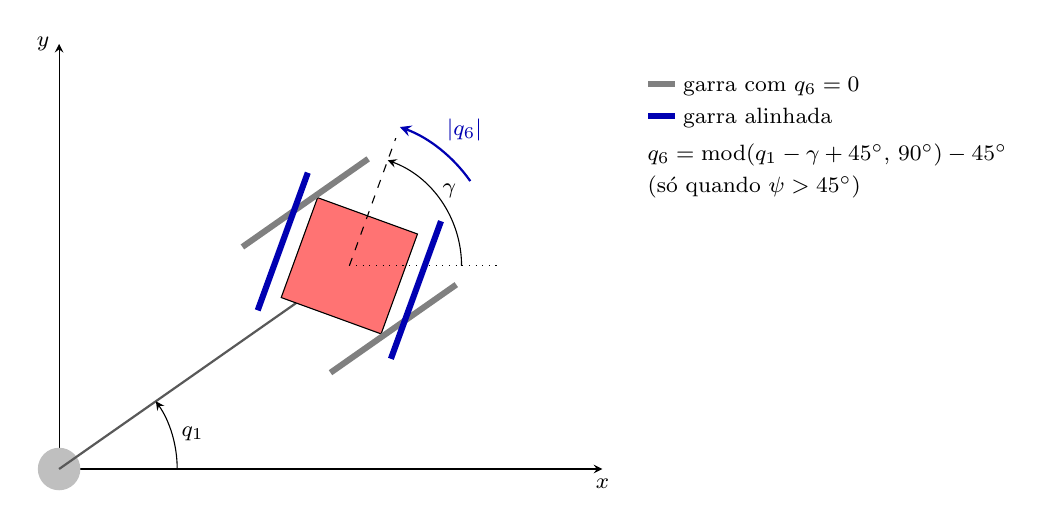
\begin{tikzpicture}[scale=1.5, >=stealth, every node/.style={font=\footnotesize}]
  \def\qa{35}   % direção do braço (q1, esboço)
  \def\ga{70}   % rotação da peça (gamma, esboço)
  % eixos da base
  \draw[->, thin] (0,0) -- (4.6,0) node[below] {$x$};
  \draw[->, thin] (0,0) -- (0,3.6) node[left] {$y$};
  \fill[gray!50] (0,0) circle (0.18);
  % direção do braço
  \draw[gray!70!black, thick] (0,0) -- (\qa:3.0);
  \draw[->, thin] (1.0,0) arc (0:\qa:1.0) node[midway, right] {$q_1$};
  % peça rodada de gamma, centrada no fim do braço
  \begin{scope}[shift={(\qa:3.0)}]
    \begin{scope}[rotate=\ga]
      \fill[red!55] (-0.45,-0.45) rectangle (0.45,0.45);
      \draw (-0.45,-0.45) rectangle (0.45,0.45);
      \draw[thin, dashed] (0,0) -- (1.15,0);
    \end{scope}
    \draw[thin, dotted] (0,0) -- (1.25,0);
    \draw[->, thin] (0.95,0) arc (0:\ga:0.95) node[pos=0.6, right] {$\gamma$};
    % garra na orientação neutra (segue q1)
    \begin{scope}[rotate=\qa]
      \draw[gray, line width=2.2pt] (-0.65,-0.65) -- (0.65,-0.65);
      \draw[gray, line width=2.2pt] (-0.65,0.65) -- (0.65,0.65);
    \end{scope}
    % garra alinhada com a peça
    \begin{scope}[rotate=\ga]
      \draw[blue!70!black, line width=2.2pt] (-0.62,-0.6) -- (0.62,-0.6);
      \draw[blue!70!black, line width=2.2pt] (-0.62,0.6) -- (0.62,0.6);
    \end{scope}
    \draw[->, blue!70!black, thick] (\qa:1.25) arc (\qa:\ga:1.25) node[pos=0.5, above right=-1pt] {$|q_6|$};
  \end{scope}
  % legenda
  \node[align=left, anchor=north west] at (4.9,3.4) {%
    \textcolor{gray}{\rule[0.5ex]{10pt}{2pt}} garra com $q_6 = 0$\\[2pt]
    \textcolor{blue!70!black}{\rule[0.5ex]{10pt}{2pt}} garra alinhada\\[4pt]
    $q_6 = \mathrm{mod}(q_1 - \gamma + 45^\circ,\, 90^\circ) - 45^\circ$\\[2pt]
    (só quando $\psi > 45^\circ$)};
\end{tikzpicture}